\begin{titlepage}
\begin{center}
\begin{textblock*}{5cm}(1cm,2.cm) % {block width} (coords)
        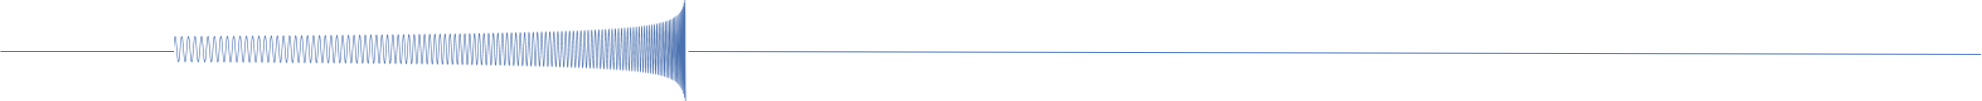
\includegraphics[width=19cm,height=1cm]{figures/Introduction/title-WF.png} % Replace with your image file
\end{textblock*}

\begin{textblock*}{5cm}(1cm, \textheight+4.2cm) % {block width} (coords)
        \reflectbox{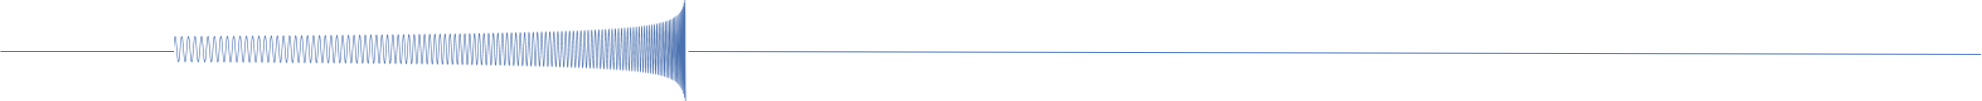
\includegraphics[width=19cm,height=1cm]{figures/Introduction/title-WF.png}} % Replace with your image file
\end{textblock*}


%\begin{textblock*}{5cm}(1cm,2.cm) % {block width} (coords)
%        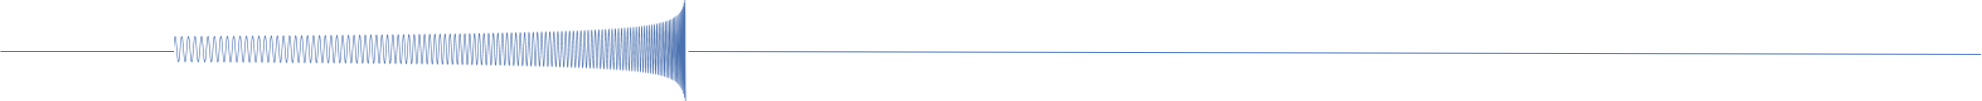
\includegraphics[width=2cm]{figures/Introduction/title-WF.png} % Replace with your image file
%\end{textblock*}

%\begin{textblock*}{5cm}(\textwidth+1cm, \textheight+4.5cm) % {block width} (coords)
%        \reflectbox{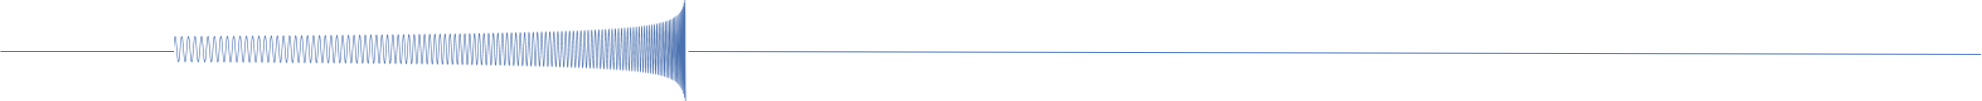
\includegraphics[width=2cm]{figures/Introduction/title-WF.png}} % Replace with your image file
%\end{textblock*}



\includegraphics[width=\textwidth]{assets/logo_band_2.png}\par
\vspace{2cm}

{\Large{\textcolor{mycolor}{Unveiling the Cosmos}: Advanced Gravitational Wave Searches for Eccentric and Precessing Binary Mergers and Their Astrophysical Implications
}}
\vfill
Von der QUEST-Leibniz-Forschungsschule\par
%Fakultät für Mathematik und Physik\par
der Gottfried Wilhelm Leibniz Universität Hannover\par
\vspace{1cm}
zur Erlangung des akademischen Grades\par
\textbf{Doktor der Naturwissenschaften}\par
\textbf{Dr. rer. nat.}\par
\vspace{1cm}
vorgelegte Dissertation von\par
\vfill
{\Large{Rahul Dhurkunde}}\par
%geboren am 28.12.1995
\vfill
{\Large{2024}}
\end{center}
\end{titlepage}
\clearpage
\thispagestyle{empty}
